\documentclass[14pt,fleqn]{article}
\usepackage{graphicx}
\usepackage[T1]{fontenc}
\usepackage[utf8]{inputenc}
\usepackage[french]{babel}
\usepackage{amsmath}
\usepackage{amssymb}
\usepackage{amscd}
\usepackage{latexsym}
\usepackage{tabularx}
\usepackage{a4wide}
%\usepackage{here}
\usepackage{enumerate}
%\usepackage{subfigure}
%\usepackage{stmaryrd}
%\usepackage{vmargin}
\usepackage{url}
\usepackage{marvosym} % Pour les euros

\usepackage{float}
\usepackage{subfig}
%\usepackage[textwidth=16cm,textheight=23cm,includefoot]{geometry}


%\renewcommand{\baselinestretch}{1.05}\small\normalsize


\newtheorem{theorem}{Theorem}
\newtheorem{conjecture}[theorem]{Conjecture}
\newtheorem{question}{Question}

\begin{document}

 \begin{figure}[H]
  \centering
  \subfloat  
{
\includegraphics[scale=1]{iflogo-azur-sable-150x60_0.png}  
}
 \hfill
  \subfloat
  {
\includegraphics[scale=.4]{gscop.png}  
}

\end{figure}


\begin{center}
\line(1,0){450}

\vspace{0.2in}
{\huge \bf ToFu: Topologie eFfective et calcUl}
\vspace{0.2in}
\line(1,0){450}
\bigskip

{\Large Projet équipe-action  \\
Mathematics: from Fundamentals to Applications}
\\

\end{center}



\begin{figure}[H]
\begin{center}
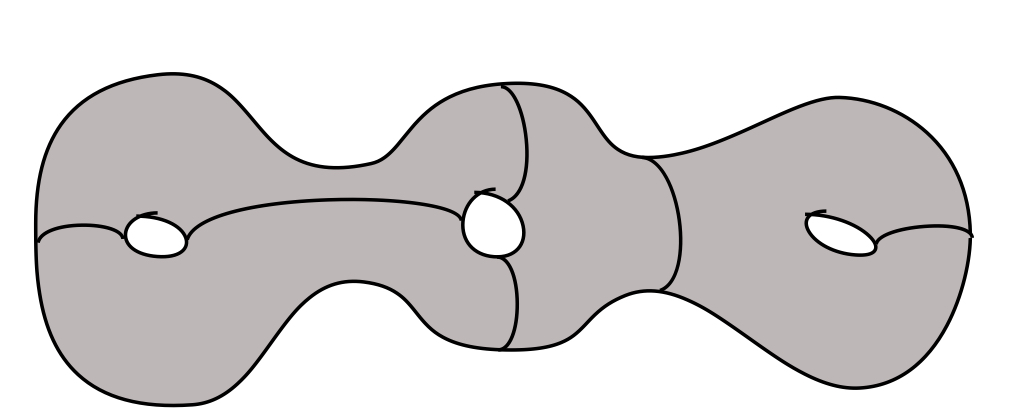
\includegraphics[scale=.25]{IMG_5383.jpg}
\end{center} 
\end{figure}

\newpage

\begin{document}

 \begin{figure}[H]
  \centering
  \subfloat  
{\includegraphics[scale=1]{tree1.png}  
}
 \hfill
  \subfloat
  {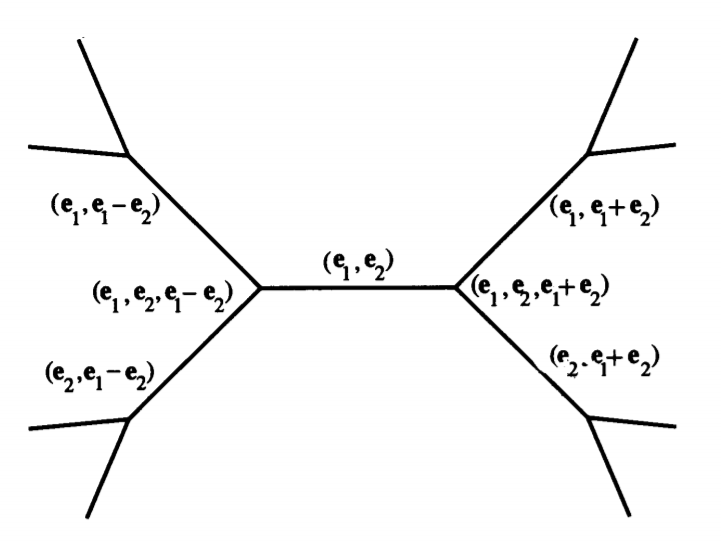
\includegraphics[scale=.4]{tree2.png}  
}

\end{figure}




\end{document}